\documentclass[10pt, letterpaper]{article}

% Inhaltsverzeichnis für Pakettypen (nur für Übersicht im Header, wird nicht im Dokument angezeigt)
% 1. Seitenlayout und Ränder
% 2. Sprache und Zeichensatz
% 3. Mathematik und Theorem-Umgebungen
% 4. Eigene Makros
% 5. Diagramme und Grafiken
% 6. Tabellen und Aufzählungen
% 7. Inhaltsverzeichnis
% 8. Abschnittsüberschriften
% 9. Abstrakt-Umgebung
% 10. Todos/Notizen
% 11. Rahmen/Box-Umgebungen
% 12. Python-Integration
% 13. Literaturverwaltung
% 14. Hyperlinks
% 15. Absatzeinstellungen
% 16. Umgebungen
% 17  Graphik
% 18  Extra
% 00. Titel und Autor

% --- 1. Seitenlayout und Ränder ---
\usepackage[margin=3cm]{geometry}

% --- 2. Sprache und Zeichensatz ---
\usepackage[english]{babel}
\usepackage[T1]{fontenc}
\usepackage[utf8]{inputenc}

% --- 3. Mathematik und Theorem-Umgebungen ---
\usepackage{amsmath, amssymb, amsthm}
\usepackage{mathrsfs}
\DeclareMathOperator{\WF}{WF}

% --- 4. Eigene Makros ---
\usepackage{xcolor}
\newcommand{\SKP}{\langle\cdot,\cdot\rangle}
\newcommand{\R}{\mathbb{R}}
\newcommand{\N}{\mathbb{N}}
\newcommand{\Q}{\mathbb{Q}}
\newcommand{\Z}{\mathbb{Z}}
\newcommand{\C}{\mathbb{C}}
\newcommand{\entwurf}[1]{\textcolor{red}{#1}}

% --- 5. Diagramme und Grafiken ---
\usepackage{graphicx}
\usepackage{tikz}
\usetikzlibrary{decorations.pathreplacing, arrows.meta, positioning}
\usepackage{tikz-cd}

% --- 6. Tabellen und Aufzählungen ---
\usepackage{enumitem}
\setlist[itemize]{left=0.5cm}

\newenvironment{romanenum}[1][]
  {%
    \ifx&#1&
    \else
      \textbf{#1}\quad
    \fi
    \begin{enumerate}[label=\roman*)]
  }
  {%
    \end{enumerate}%
  }

% --- 7. Inhaltsverzeichnis ---
\usepackage{tocloft}
\renewcommand{\cftsecfont}{\footnotesize}
\renewcommand{\cftsubsecfont}{\footnotesize}
\renewcommand{\cftsubsubsecfont}{\footnotesize}
\renewcommand{\cftsecpagefont}{\footnotesize}
\renewcommand{\cftsubsecpagefont}{\footnotesize}
\renewcommand{\cftsubsubsecpagefont}{\footnotesize}
\usepackage{etoc}

% --- 8. Abschnittsüberschriften ---
\usepackage{titlesec}
\titleformat{\section}{\normalfont\large\bfseries}{\thesection}{1em}{}
\titleformat{\subsection}{\normalfont\normalsize\bfseries}{\thesubsection}{0.5em}{}
\titleformat{\subsubsection}{\normalfont\normalsize\bfseries}{\thesubsubsection}{0.5em}{}
\setcounter{secnumdepth}{4}

% --- 9. Abstrakt-Umgebung ---
\usepackage{changepage}
\renewenvironment{abstract}
  {
    \begin{adjustwidth}{1.5cm}{1.5cm}
    \small
    \textsc{Abstract. –}%
  }
  {
    \end{adjustwidth}
  }

% --- 10. Todos/Notizen ---
\usepackage{todonotes}

% --- 11. Rahmen/Box-Umgebungen ---
\usepackage{mdframed}
\usepackage{tcolorbox}
\colorlet{shadecolor}{gray!25}

\newenvironment{customTheorem}
  {\vspace{10pt}%
   \begin{mdframed}[
     backgroundcolor=gray!20,
     linewidth=0pt,
     innertopmargin=10pt,
     innerbottommargin=10pt,
     skipabove=\dimexpr\topsep+\ht\strutbox\relax,
     skipbelow=\topsep,
   ]}
  {\end{mdframed}
   \vspace{10pt}%
  }

% --- 12. Python-Integration ---
% (Deaktiviert in dieser Version, aktiviere bei Bedarf)
% \usepackage{pythontex}
% \usepackage[makestderr]{pythontex}

% --- 13. Literaturverwaltung ---
\usepackage{csquotes}
\usepackage[backend=biber, style=alphabetic, citestyle=alphabetic]{biblatex}
\addbibresource{bibliography.bib}

% --- 14. Hyperlinks ---
\usepackage{hyperref}
\hypersetup{
  colorlinks   = true,
  urlcolor     = blue,
  linkcolor    = blue,
  citecolor    = blue,
  frenchlinks  = true
}

% --- 15. Absatzeinstellungen ---
\usepackage[parfill]{parskip}
\sloppy

% --- 16. Umgebungen ---
\usepackage{thmtools}

\newcommand{\CustomHeading}[3]{%
  \par\medskip\noindent%
  \textbf{#1 #2} \textnormal{(#3)}.\enskip%
}

\newenvironment{DEF}[2]{\CustomHeading{Definition}{#1}{#2}}{}
\newenvironment{PROP}[2]{\CustomHeading{Proposition}{#1}{#2}}{}
\newenvironment{THEO}[2]{\CustomHeading{Theorem}{#1}{#2}}{}
\newenvironment{LEM}[2]{\CustomHeading{Lemma}{#1}{#2}}{}
\newenvironment{KORO}[2]{\CustomHeading{Corollar}{#1}{#2}}{}
\newenvironment{REM}[2]{\CustomHeading{Remark}{#1}{#2}}{}
\newenvironment{EXA}[2]{\CustomHeading{Example}{#1}{#2}}{}
\newenvironment{STUD}[2]{\CustomHeading{Study}{#1}{#2}}{}
\newenvironment{CONC}[2]{\CustomHeading{Concept}{#1}{#2}}{}

\newenvironment{PROOF}
  {\begin{proof}}%
{\end{proof}}

% --- Unit Umgebung für Source-Inhalte ---
\usepackage{mdframed}
\newmdenv[
  linewidth=1pt,
  topline=false,
  bottomline=false,
  rightline=false,
  leftmargin=0cm,
  rightmargin=0cm,
  skipabove=10pt,
  skipbelow=10pt,
  innertopmargin=0.5\baselineskip,
  innerbottommargin=0.5\baselineskip,
  backgroundcolor=gray!10,
  linecolor=gray
]{unitbox}

\newenvironment{unit}[1]
  {\begin{unitbox}\textbf{Unit #1}\par\smallskip}
  {\end{unitbox}}

% --- 17. Graphik ---
\usepackage{graphicx}
\graphicspath{ {./images/} }
\usepackage[export]{adjustbox}

% --- 18. Extras ---
\usepackage{stmaryrd}
\usepackage{bbold}  % falls du athbb{1} nutzen willst

% --- 00. Titel und Autor ---
\title{Mein Titel}
\author{Tim Jaschik}
\date{\today}



%New command to display footnote whose markers will always be hidden
\let\svthefootnote\thefootnote
\newcommand\blfootnotetext[1]{%
  \let\thefootnote\relax\footnote{#1}%
  \addtocounter{footnote}{-1}%
  \let\thefootnote\svthefootnote%
}

%Overriding the \footnotetext command to hide the marker if its value is `0`
\let\svfootnotetext\footnotetext
\renewcommand\footnotetext[2][?]{%
  \if\relax#1\relax%
    \ifnum\value{footnote}=0\blfootnotetext{#2}\else\svfootnotetext{#2}\fi%
  \else%
    \if?#1\ifnum\value{footnote}=0\blfootnotetext{#2}\else\svfootnotetext{#2}\fi%
    \else\svfootnotetext[#1]{#2}\fi%
  \fi
}


\begin{document}

\maketitle
\rule{\textwidth}{0.5pt}
\begin{abstract}
Kurze Beschreibung …
\end{abstract}
\rule{\textwidth}{0.5pt}
\vspace{0.5cm}

\tableofcontents

\pagebreak


\begin{abstract}
This is meant to be a gentle introduction to the theory of knots, aimed specifically at physicists who want some background to Freedman and He's work (1991) relating asymptotic crossing number of knots to estimates of the energy in a knotted divergencefree flow.
\end{abstract}


\section{Knotting and unknotting}
DEFINITION 1. A knot $K$ in a smooth 3-manifold $M^{3}$ is the image of a smooth non-singular imbedding $f: S^{1} \rightarrow M^{3}$.

Here "non-singular" means that the derivative of f is non-zero and is included only to exclude the sort of pathological behavior shown in figure 1.

Two knots are regarded as equivalent, or isotopic, if you can move one to the other in $M^{3}$. Explicitly

DEFINITION 2. Two knots $K$ and $K^{\prime}$ are isotopic (write $K \sim K^{\prime}$ ) if there is a smooth non-singular level-preserving embedding $F: S^{1} \times I \rightarrow M \times I$ such that $F\left(S^{1} \times\{0\}\right)=K$ and $F\left(S^{1} \times\{1\}\right)=K^{\prime}$.

Once again non-singular is thrown in to eliminate pathological behavior. In particular, without it, all knots are unknotted! (See figure 2.)

Although these definitions are the most useful from the point of view of differential topology, the pathologies above often tempt topologists to think in a somewhat different category, called the PL category. In this category $M^{3}$ has a local linear structure, and in it knots are closed polygonal curves. From the point of view of the topology of the knot, these viewpoints are

\footnotetext{\begin{itemize}
  \item Research supported in part by a National Science Foundation Grant
\end{itemize}
}
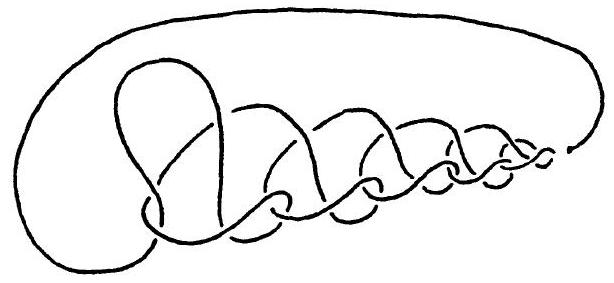
\includegraphics[scale=0.2, center]{2025_05_21_037de704f595ce642d3eg-077(1)}

Fig. 1. Singular, or "wild" point.\\
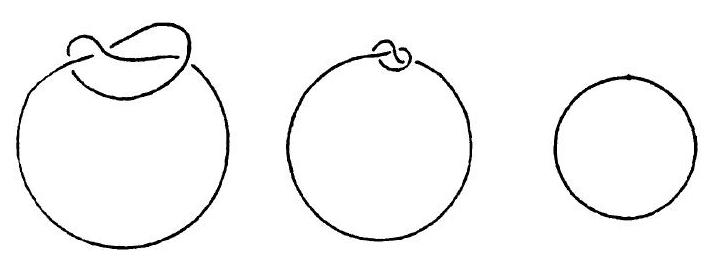
\includegraphics[scale=0.2, center]{2025_05_21_037de704f595ce642d3eg-077}

Fig. 2. A singular unknotting.\\
identical, but of course the corners may play havoc with any arguments involving the knot's differential structure (e. g. the curvature of the knot.)

Here we'll only be concerned with knots in 3 -space. Since topologists have a preference for compact spaces, often they secretly regard the knots as lying in the 3 -sphere. For most elementary purposes, the distinction between $R^{3}$ and $S^{3}$ is unimportant, for the difference is a single point at infinity. This point can be taken to be disjoint from the knot and its isotopies.

An advantage of working with knots in the 3 -sphere (or 3 -space) instead of an arbitrary 3 -manifold, is the following theorem, called the Alexander trick:

THEOREM 1. $K \sim K^{\prime}$ in $S^{3}$ if and only if there is an orientation preserving diffeomorphism of $S^{3}$ carrying $K$ to $K^{\prime}$.

DEFINITION 3. $K$ is unknotted (or the unknot) if it is isotopic to $S^{1} \subset S^{3}$ (equivalently, to the round circle in the plane in 9 -space).

Here's an equivalent formulation:\\
THEOREM 2. $K$ is unknotted in $S^{3}$ if and only if $K$ bounds a smooth disk in $S^{3}$.\\
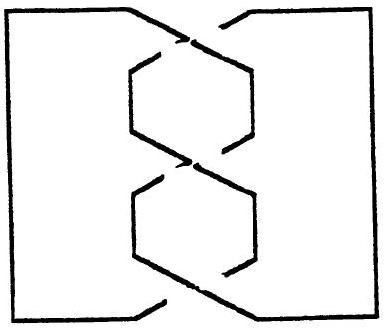
\includegraphics[scale=0.2, center]{2025_05_21_037de704f595ce642d3eg-078(1)}

Fig. 3. Polyhedral picture of trefoil knot.\\
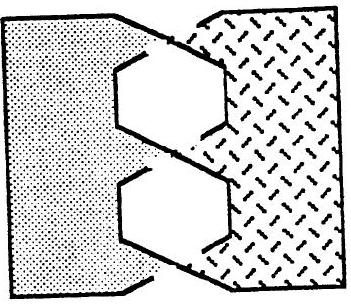
\includegraphics[scale=0.2, center]{2025_05_21_037de704f595ce642d3eg-078}

Fig. 4. Seifert surface for the trefoil knot.

Proof: Suppose $K$ is unknotted in $S^{3}$, so there is a diffeomorphism of $S^{3}$ taking $K$ to $S^{1} \subset S^{3}$. Now $S^{1}$ bounds a hemisphere of $S^{2} \subset S^{3}$; carry the hemisphere back by the inverse of the diffeomorphism.

Conversely, suppose $K$ bounds a smooth disk $D$ in $S^{3}$. A tiny neighborhood of the center of $D$ is essentially a flat round disk $D^{\prime}$, whose boundary is a round circle. The annulus $D-D^{\prime}$ then isotopes $K=\partial D$ to $\partial D^{\prime}$.



\section{Seifert surfaces and knot genus}

Although only the unknot bounds a disk, a general statement holds for all knots:

THEOREM 3. (Seifert) Any knot bounds some orientable surface in $S^{3}$.

Such a surface is called a Seifert surface of the knot. A Seifert surface of a knot isn't unique, even up to isotopy, for one can always attach tubes to a given surface and make it more complicated. Even if we restrict to the simplest possible Seifert surface, there are knots with infinitely many non-isotopic such surfaces. Nonetheless, the complexity of such surfaces is a useful indicator of the complexity of the knot.\\
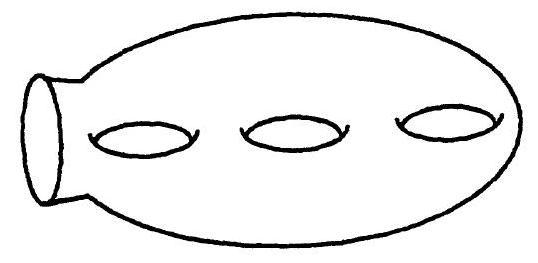
\includegraphics[scale=0.2, center]{2025_05_21_037de704f595ce642d3eg-079}

Fig. 5. A genus three surface.\\
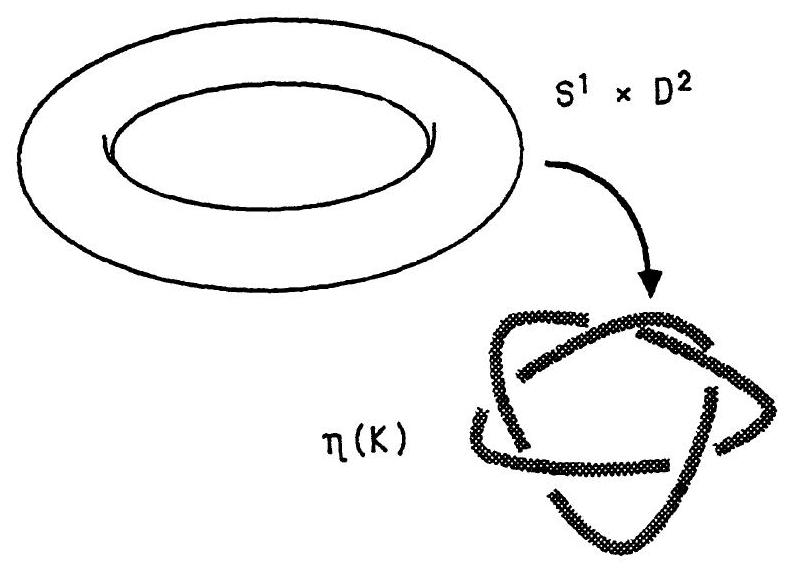
\includegraphics[scale=0.2, center]{2025_05_21_037de704f595ce642d3eg-079(1)}

Fig. 6. A regular neighborhood $\eta$ of a knot $K$.

DEFINITION 4. A knot $K$ in $S^{3}$ has genus $n$ if it bounds an orientable surface of genus $n$, but not one of genus $n-1$.

Note: The Seifert surface in figure 4 and the following corollary show that the trefoil knot has genus one.

COROLLARY 1. A knot $K$ has genus 0 if and only if it is unknotted.\\
Proof: A genus 0 surface with one boundary component is a disk.\\
THEOREM 4. A smooth knot $K$ has a tubular neighborhood. That is, there is a neighborhood $\eta(K)$ of $K$ so that the pair $(\eta(K) ; K)$ is diffeomorphic to $S^{1} \times\left(D^{2}, 0\right)$.

DEFINITION 5. The boundary $\partial \eta(K)$ of a tubular neighborhood of $K$ is diffeomorphic to the torus $S^{1} \times S^{1}$. It contains two special circles:\\
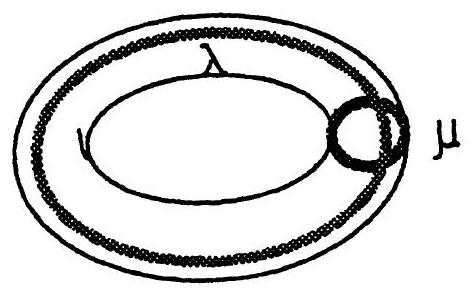
\includegraphics[scale=0.2, center]{2025_05_21_037de704f595ce642d3eg-080}

Fig. 7. Meridian $\mu$ and longitude $\lambda$.

The meridian is the boundary of a cross-sectional disk $\{*\} \times D^{2} \subset S^{1} \times D^{2}$ and is denoted $\mu$.

The longitude is denoted $\lambda$ and is the boundary of a Seifert surface.

THEOREM 5. The meridian and longitude of a knot $K$ are uniquely defined in $\partial \eta(K)$ up to isotopy.

Proof: The harder part is showing the uniqueness of $\lambda$. This can be done by studying the arcs of intersection of two different Seifert surfaces. Alternately, there's an easy proof from algebraic topology. First note that two simple closed curves $c$ and $c^{\prime}$ imbedded in $S^{1} \times S^{1}$ are isotopic if and only if the algebraic intersection $c \cdot c^{\prime}$ is trivial. If $S$ and $S^{\prime}$ are two Seifert surfaces for $K$, then $\partial S \cdot \partial S^{\prime}=\partial\left[S \cdot S^{\prime}\right]$. But $S \cdot S^{\prime}$ is in $H_{1}(M, \partial M)$, which is trivial.

Remark: The natural choice of circles $\lambda$ and $\mu$ then allows us to describe any simple closed curve on $\partial \eta(K)$ by a number in the extended rationals $Q \cup(\infty)$. The curve homologous to $p \mu+q \lambda$ we associate with the rational number $p / q$. (e. g. $\mu \rightarrow \infty$ ).



\section{Winding, (w)rapping, and satellites}

DEFINITION 6. Suppose $k$ is a knot in $S^{1} \times D^{2}$. Then the winding number of $k$, denoted $w(k)$, is the algebraic intersection $k \cdot D^{2}$ of $k$ with a crosssectional disk $\{*\} \times D^{2}$. Here algebraic intersection means that an intersection in one direction across the disk will cancel an intersection going in the other direction. In contrast, the wrapping number $r(k)$ of $k$ is the number of times which $k$ intersects $D^{2}$ (regardless of direction), minimized by isotopies of $k$ in $S^{1} \times D^{2}$.

Figure 8 illustrates a knot which has winding number zero, but wrapping number 2.\\
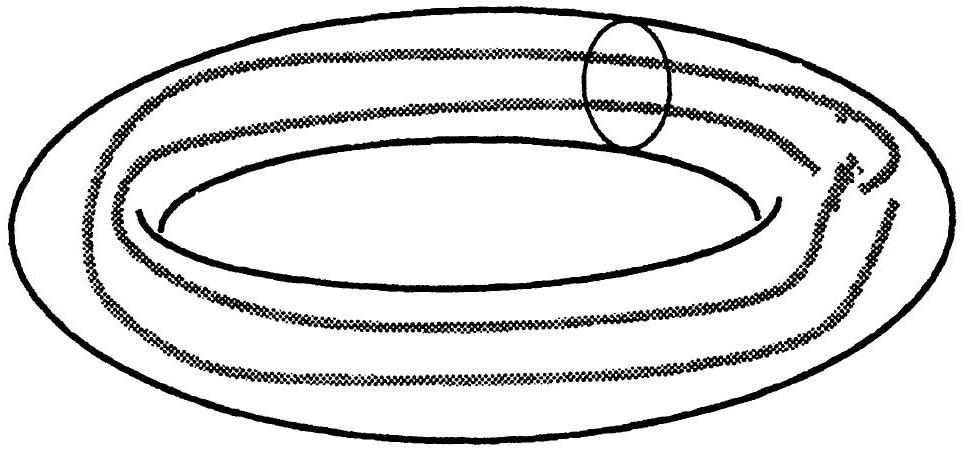
\includegraphics[scale=0.2, center]{2025_05_21_037de704f595ce642d3eg-081}

Fig. 8. How to "double" a knot.

One way of creating new knots is by imbedding simple closed curves in the tubular neighborhoods of other knots. Specifically, suppose $K$ is a knot in $S^{3}$. We would like to make the following preliminary definition: $k$ is a satellite of $K$ if $k \subset \eta(K)$.

But a moments reflection shows that some caution is in order. Here are some problems:\\
a) Any knot is a satellite of the unknot. Indeed, put a little loop $l$ around a given knot $k$. Then the complement of $l$ in $S^{3}$ is itself a (very large) regular neighborhood of an unnamed unknot. Since $k$ lies in the complement of $l, k$ would automatically be a satellite of the unknot.\\
b) $k$ may be isotopic to $K$ in $\eta(K)$, so in effect $k$ is $K$.\\
c) If $r(k)=0$ then $k$ misses a cross-sectional disk of $\eta(K)$. The complement of such a disk in $\eta(K)$ is just a 3-ball. Any knot can be isotoped into any 3-ball (just shrink $R^{3}$ ), so if we were to allow $r(k)=0$, then any knot would be a satellite of any other!

With these things in mind we make the final

DEFINITION 7. a) $k \subset \eta(K)$ is a satellite of $K$ if $r(k) \neq 0$ and $k$ is not isotopic to $K$ in $\eta(K)$.\\
b) $k$ is a satellite knot if it's a satellite of $K$, for $K$ not the unknot.\\
(Note that a satellite of the unknot is not necessarily a satellite knot!)

DEFINITION 8. Suppose $k$ is a satellite of $K$. The pattern of $k$ is $h(k)$, for $h: \eta(K) \rightarrow S^{1} \times D^{2}$. In general, ambiguity in the choice of $h$ from possible twisting of $S^{1} \times D^{2}$ would result in ambiguity of the pattern. This can be circumvented by insisting that the longitude in $\eta(K)$ go to $S^{1} \times\{*\}$, for some point * in $\partial D^{2}$.\\
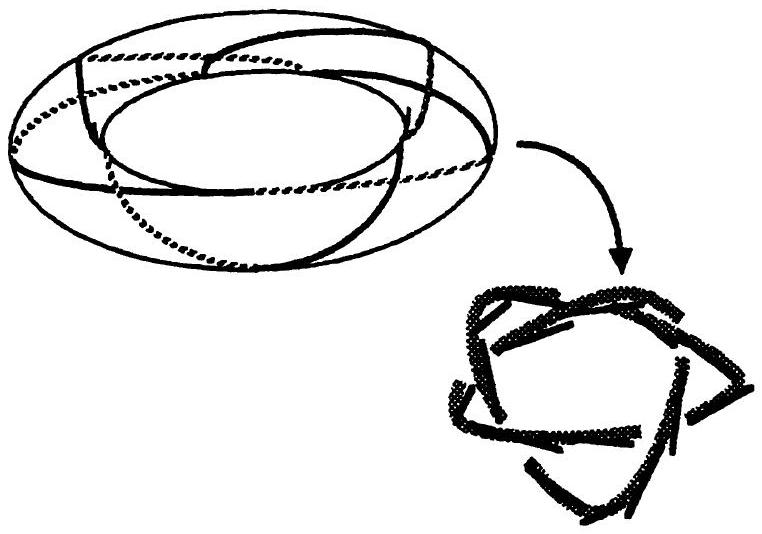
\includegraphics[scale=0.2, center]{2025_05_21_037de704f595ce642d3eg-082}

Fig. 9. How to cable a knot.

Some important examples of satellite knots are those obtained from the following patterns:

\begin{enumerate}
  \item Double of a knot: Pick the simplest pattern with $w(k)=0, r(k)=2$. See figure 8.
  \item Parallels of a knot: Pick for $k$ several parallel copies of the core knot $K$. (Strictly speaking, this is a link, since there are several components).
  \item Cables of a knot: Let the pattern be the torus knot on $\partial \eta(K)$. See figure 9.
\end{enumerate}

In some sense, detecting satellite knots is fairly easy, thanks to the following theorem of Alexander.

THEOREM 6. Any $T^{2} \subset S^{3}$ bounds a solid torus on at least one side.\\
COROLLARY 2. If there's a torus $T^{2} \subset S^{3}-k$ which is not parallel to $\partial \eta(k)$ and doesn't bound a solid torus in $S^{3}-k$, then $k$ is a satellite knot.



\section{Band sums and connected sums of knots}

DEFINITION 9. A link is an embedded disjoint union of circles in $S^{3}$. A link is split if it's the distant union of two proper sublinks.

DEFINITION 10. The band-sum $K \#_{b} K^{\prime}$ is obtained by banding together distant copies of $K$ and $K^{\prime}$.

DEFINITION 11. The connected sum $K \# K^{\prime}$ is obtained by banding together distant copies of $K$ and $K^{\prime}$ via a band crossing a splitting sphere once. $K \# K^{\prime}$ is called a composite knot.\\
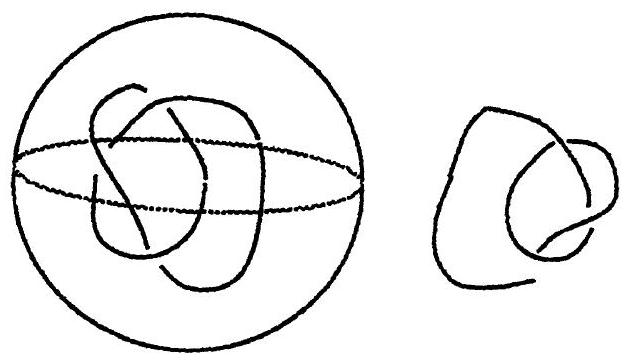
\includegraphics[scale=0.2, center]{2025_05_21_037de704f595ce642d3eg-083(1)}

Fig. 10. A split link.\\
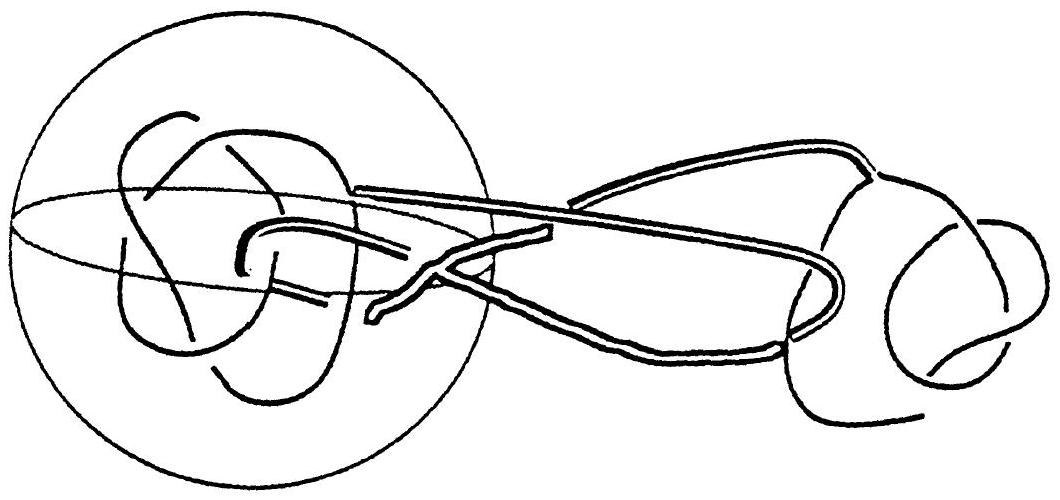
\includegraphics[scale=0.2, center]{2025_05_21_037de704f595ce642d3eg-083(2)}

Fig. 11. The band sum $K \#_{b} K^{\prime}$ of knots.\\
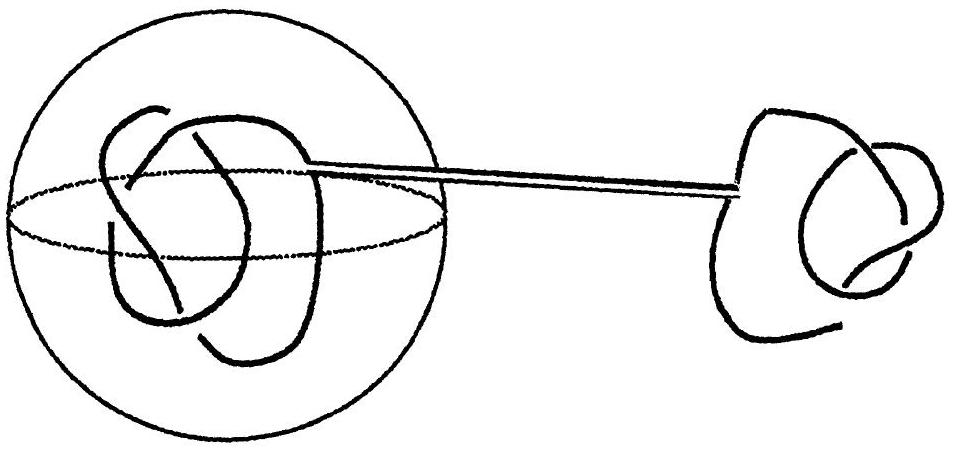
\includegraphics[scale=0.2, center]{2025_05_21_037de704f595ce642d3eg-083}

Fig. 12. The connected sum $K \# K^{\prime}$ of knots.

In general, the knot obtained from $K \#_{b} K^{\prime}$ depends heavily on the choice of $b$ as well as that of $K$ and $K^{\prime}$. Not so, when we consider just the connected sum. Indeed

THEOREM 7. $K \# K^{\prime}$ is well-defined.

Proof: : The proof is surprisingly simple: Suppose in figure 12 a band had been chosen so that it intersected the sphere once, but the part of the band outside the sphere was complicated. Just shrink the ball on the left, containing one summand, down to the size of a pea, and unravel the band. Then blow the ball up again. Now the band is straight outside the ball. Repeat the process using a ball around the other summand to straighten out the band inside the sphere.

In light of this theorem, we can regard the connected sum as a binary operation on the set of knots. It's easy to see that the operation is commutative ( $K_{1} \# K_{2}$ is isotopic to $K_{2} \# K_{1}$ ), associative ( $\left(K_{1} \# K_{2}\right) \# K_{3}$ is isotopic to $K_{1} \#\left(K_{2} \# K_{3}\right)$ ) and that the unknot $O$ is an identity element ( $K \# O$ is isotopic to $K$ ). To a mathematician this means that \# induces a "commutative monoid structure". To be a commutative group, all that's missing is the existence of an inverse. Hence we get the natural question: Given a knot $K$, is there a knot $K^{\prime}$ such that $K \# K^{\prime}=O$ ?

As an applied problem, this can be translated to: If a garden hose is knotted, is there a way of tying another knot in an end of the hose, so that when slid down to the first knot, the two cancel and the hose is unknotted. Experienced gardeners know that this is impossible, but the mathematician requires proof. In fact, it's an elementary corollary of the following more general:

THEOREM 8. For $K$ and $K^{\prime}$ two knots in $S^{3}$, genus $\left(K \# K^{\prime}\right)=\operatorname{genus}(K)+$ genus ( $K^{\prime}$ ).

Proof: 1) The inequality genus ( $K \# K^{\prime}$ ) $\leq \operatorname{genus}(K)+\operatorname{genus}\left(K^{\prime}\right)$ is immediate: If $S$ and $S^{\prime}$ are minimal genus Seifert surfaces for $K$ and $K^{\prime}$ respectively, just glue an arc on $\partial S=K$ to an arc on $\partial S^{\prime}=K^{\prime}$. (See figure 13.) The genus of the resulting surface $T$ is genus $(K)+$ genus $\left(K^{\prime}\right)$, and $\partial T=K \# K^{\prime}$. $T$ may not be of minimal genus among all Seifert surfaces of $K \# K^{\prime}$, so we only get an inequality, not an equality.\\
2) The inequality genus $\left(K \# K^{\prime}\right) \geq \operatorname{genus}(K)+\operatorname{genus}\left(K^{\prime}\right)$ is more difficult. What we need to show is that given a Seifert surface $T$ for $K \# K^{\prime}$, it can be viewed, as above, as a Seifert surfaces for $K$ and $K^{\prime}$ glued together along an arc. The idea is to start with $T$ and modify it in a way that does not increase genus but so that it will eventually intersect a sphere $S^{2}$ separating $K$ from $K^{\prime}$ in a single arc. Now $S^{2}-\left(K \# K^{\prime}\right)$ is an annulus $A$ whose ends are\\
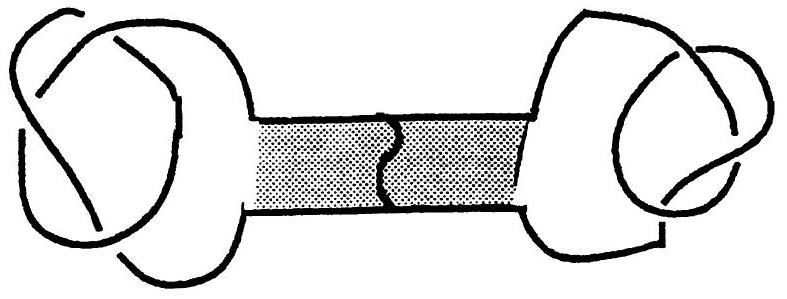
\includegraphics[scale=0.2, center]{2025_05_21_037de704f595ce642d3eg-085(1)}

Fig. 13. Gluing together Seifert surfaces of $K$ and $K^{\prime}$.\\
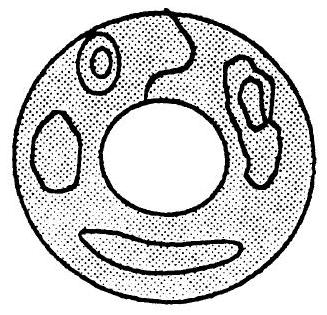
\includegraphics[scale=0.2, center]{2025_05_21_037de704f595ce642d3eg-085}

Fig. 14. $T \cap A$\\
meridians of $K \# K^{\prime}$. Since $\partial T=K \# K^{\prime}, T \cap A$ is a 1-manifold with precisely two ends, one at each end of $A$. Viewed in $A$, this means that either $T \cap A$ is a single arc, and we're done, or $T \cap A$ contains also a bunch of circles (see figure 14).

In the latter case, at least one component of $T \cap A$ bounds a disk in $A$ containing no other component of $T \cap A$. Figure 15 shows how to use this disk to modify $T$ so that this component, and maybe more, is removed from $T \cap A$.

The operation may decrease, but won't increase, the genus of $T$. After sufficiently many such operations, all circles of intersection are removed.

Remark: It is a much deeper result, proven only recently (Gabai (1987), Scharlemann (1989)), that genus $\left(K \#_{b} K^{\prime}\right) \geq \operatorname{genus}(K)+\operatorname{genus}\left(K^{\prime}\right)$.\\
COROLLARY 3. (Absence of inverses) If $K \# K^{\prime}=O$ then $K=K^{\prime}=O$.\\
Proof: : Since genus $(K)+\operatorname{genus}\left(K^{\prime}\right)=0$, genus $(K)=\operatorname{genus}\left(K^{\prime}\right)=0$, so $K$ and $K^{\prime}$ are both the unknot.\\
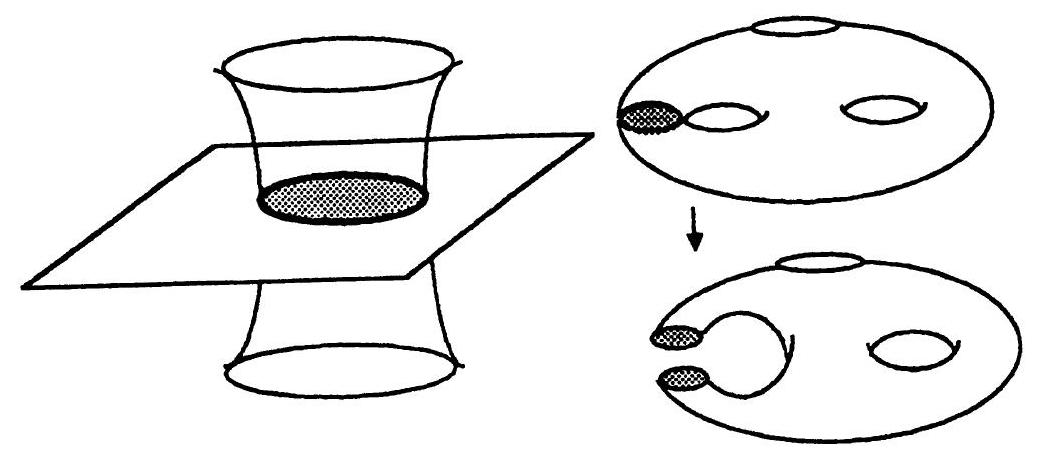
\includegraphics[scale=0.2, center]{2025_05_21_037de704f595ce642d3eg-086}

Fig. 15. "Compressing" $T$.



COROLLARY 4. Genus one knots are prime (= not composite).\\
Proof: : Suppose $\bar{K}$ is composite, so $\bar{K}=K \# K^{\prime}$, with genus $(K)$, genus $\left(K^{\prime}\right) \geq$ 1. Then genus $(\bar{K}) \geq 1+1=2$.

THEOREM 9. A knot $k$ is a satellite of a knot $K_{1}$ with $r(k)=1$ if and only if $k$ is the connected sum of $K_{1}$ with another knot $K_{0}$.

Proof: The proof is in the figure 16, which shows how $K_{0} \# K_{1}$ is imbedded in a tubular neighborhood of $K_{1}$. The illustrated torus $T$ is called a "followswallow" torus, because it follows $K_{1}$ around, but swallows $K_{0}$.


\section{Bridge number and curvature}

DEFINITION 12. The bridge number $\beta$ of a link is the minimum number of bridges needed to construct a freeway system supporting the link. The traffic rule is: you cross over each bridge exactly once, but can go under each bridge any number of times. By convention, $\beta(O)=1$ (not 0 ).

To see that this definition is symmetric, note that a path on the ground is travelled over once, though a bridge may pass over each path any number of times.

Figure 17 shows a two-bridge link, with the bridges appearing as horizontal segments.

There is an equivalent definition: If we look at the link in bridge position from the side, e. g. standing on the ground a good distance away, then the bridges can be viewed as maxima of a height function on $K$, and the paths\\
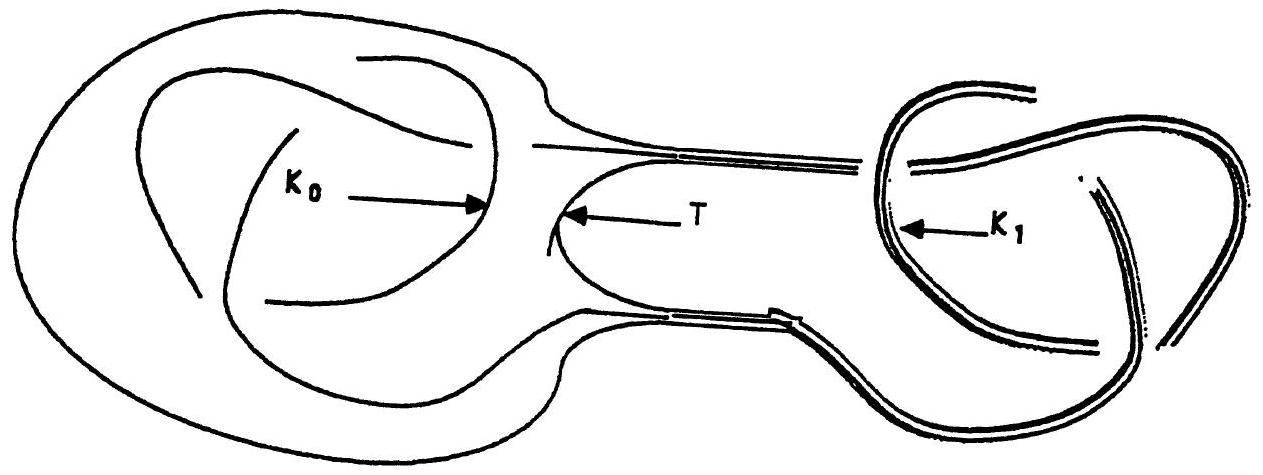
\includegraphics[scale=0.2, center]{2025_05_21_037de704f595ce642d3eg-087(1)}

Fig. 16. The follow-swallow torus.\\
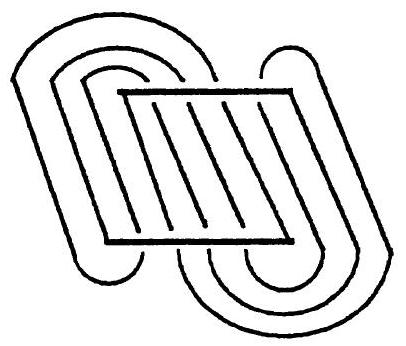
\includegraphics[scale=0.2, center]{2025_05_21_037de704f595ce642d3eg-087}

Fig. 17. A two-bridge link.\\
on the ground as minima. So we get: There's a height function on $K$ with $n$ maxima if and only if $K$ has bridge number $\leq n$.

Here's yet a third picture. Imagine taking such a height function and exaggerating it, so the knot is actually hanging from its maxima, and its minima are pegged to a lower level. Then running between the top and the bottom is a braid of $2 n$-strands. This is said to be a $2 n$-plat presentation for the link (see figure 18).

For a fourth picture, imagine a plane which cuts through the plat presentation just above the minima. Then below the plane the minima just appear as a family of unknotted arcs. What's slightly more difficult to see is that if we ignore everything below the plane, and just look at the arcs lying above the plane, they too are isotopic (as proper arcs) to a family of unknotted arcs, by sliding their end points around on the plane. So $k$ has bridge number $\leq n$ if and only if there is a plane cutting it into two families of $n$ unknotted unlinked arcs.\\
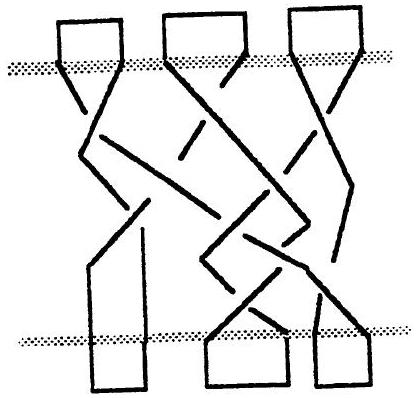
\includegraphics[scale=0.2, center]{2025_05_21_037de704f595ce642d3eg-088}

Fig. 18. A plat presentation for a three-bridge knot.\\
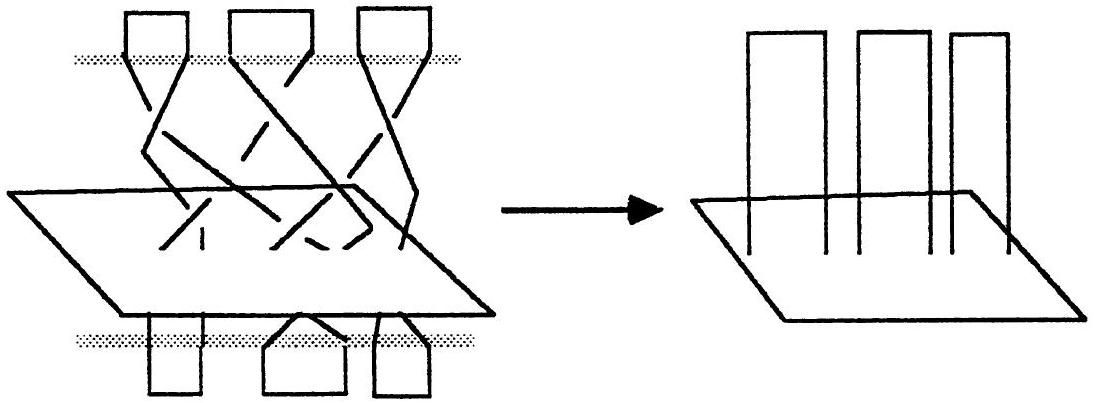
\includegraphics[scale=0.2, center]{2025_05_21_037de704f595ce642d3eg-088(1)}

Fig. 19. Trivializing arcs above the plane.

THEOREM 10. If $K$ has bridge number one then $K$ is the unknot.\\
Proof: : There is a single maxima, hence a single minima. Between these two critical points $K$ intersects each plane in two points. In each level plane, connect the two points of intersection with an arc, which can be taken to vary continuously with the level. The result is a disk whose boundary is the knot.

Here is a deep theorem of Schubert (1954). For a modern proof, see Doll (1991), where it is also shown that it's possible to define a notion of bridge number for surfaces more complicated than planes (equivalently spheres).

THEOREM 11. a) If $k$ is a satellite of $K$ then $\beta(k) \geq r(k) \cdot \beta(K)$.\\
b) $\beta\left(K_{1}\right)+\beta\left(K_{2}\right)-1=\beta\left(K_{1} \# K_{2}\right)$.

Remark: b) follows from a) by using the "follow-swallow" torus knot above.\\
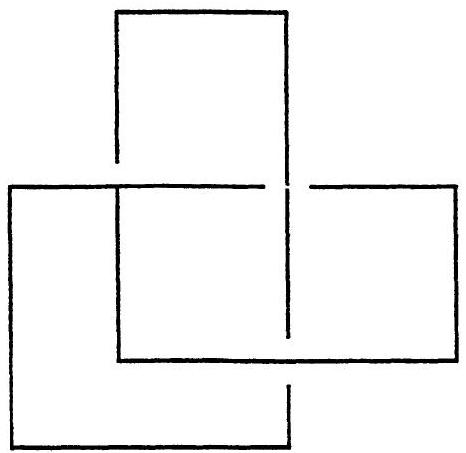
\includegraphics[scale=0.2, center]{2025_05_21_037de704f595ce642d3eg-089}

Fig. 20. A nearly flat trefoil knot, with $\kappa$ near $4 \pi$

\section*{COROLLARY 5. 2-bridge knots are prome and not satellites.}
There is a remarkable connection between the curvature of a knot and its bridge number, discovered by John Milnor (1950) (when he was a teenager!). It is interesting in its own right, but is included here also because of its prescient connection to two notions of energy for a knot. Let $\kappa(k)$ denote the total curvature of a knot $k$ in $S^{3}$. It has the following polyhedral interpretation (indeed, this motivates the definition of curvature): For $k$ a polyhedral knot in $R^{3}$, let $\kappa(k)$ denote the sum of the exterior angles at corners of $k$.

THEOREM 12. $\kappa(k) \geq 2 \pi \beta(k)$.\\
COROLLARY 6. If $\kappa(k)<4 \pi$ then $k$ is the unknot.\\
Remark: In fact, $\kappa(k) \leq 4 \pi$ implies that $k$ is unknotted. Figure 20 shows that the estimate is sharp. The total exterior angle looks just like $4 \pi$, but this is an optical illusion. At least one of the straight lines must be bent or broken slightly, raising $\kappa(k)$ above $4 \pi$.

Proof of Milnor's theorem: We'll prove the polyhedral version; the smooth version can be gotten by polyhedral approximation. Let $p_{1}, \ldots, p_{n}$ be the $n$ corners of the polyhedral approximation, and let $\alpha_{i}$ denote the exterior angle at $p_{i}$. Then $\kappa(k)=\sum \alpha_{i}$.

For any angle $\alpha$ in 3 -space, there is a circular sector of directions $\sigma_{\alpha}$ in $S^{2}$ so that a height function with gradient in that direction will have a maxima at the angle's vertex (see figure 21).

We have $\operatorname{area}\left(\sigma_{\alpha}\right) / \operatorname{area}($ sphere $)=\alpha / 2 \pi$, so $\operatorname{area}\left(\sigma_{\alpha}\right)=2 \cdot \alpha$. Let $\sigma_{i}$ denote the angle corresponding to $\alpha_{i}$. In particular the vector v is in $\sigma_{i}$ if and only if $\alpha_{i}$ is a maximum for a height function whose gradient is v. Put another way, if the number of maxima for $k$ along such a height function is $n$, then $v$ lies in $n$ of the $\sigma_{i}$. The average number of maxima appearing over\\
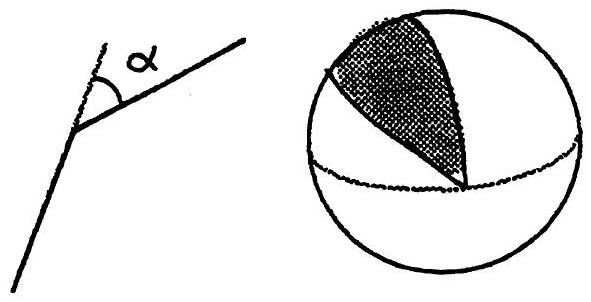
\includegraphics[scale=0.2, center]{2025_05_21_037de704f595ce642d3eg-090}

Fig. 21. A corner and its associated sphere segment.\\
all directions $\mathbf{v}$ is then simply $\sum$ area $\left(\sigma_{i}\right)$ divided by the area of the sphere, $4 \pi$. If we then let $n_{0}$ be the minimum number of maxima appearing at any direction $\mathbf{v}$, it will clearly be no larger than the average, so we have

$$
\beta(k) \leq n_{0} \leq \sum \operatorname{area}\left(\sigma_{i}\right) / 4 \pi=\left(\sum 2 \cdot \alpha_{i}\right) / 4 \pi=(\kappa(k)) / 2 \pi
$$

as required.

\section*{Connections with knot energy}
There are two connections here with notions of knot energy. The first is directly mathematical. If we imagine the knot made from an elastic straight wire, Bernoulli-Euler theory states that the amount of bending energy required to create the knot is the integral of $\kappa^{2}$ around the knot. A polyhedral approximation here is not allowed, for to create a corner requires an infinite amount of energy. This notion of energy for a knot is relatively accessible, and much is known (the definitive treatment is Langer and Singer (1985). For a knot theorist, however, the theory is ultimately disappointing. Langer and Singer show that an energy-reducing flow will always lead to self-intersections of a knot, changing its knot type. Eventually such a flow will terminate in a round circle.

The second connection is not so direct, but leads to the Freedman-He (1991) notion of average crossing number. We have seen how the total curvature of a knot describes an average bridge number for a specific position of the knot in $R^{3}$. Here the average is taken over all possible directions for a linear height functions on the knot in $R^{3}$.

Instead of the bridge number, consider another invariant of a knot $k$ in $R^{3}$. For each direction in $R^{3}$ (i. e. unit vector $\mathbf{v}$ in $S^{2}$ ), project the knot onto the plane perpendicular to $\mathbf{v}$, and count the number of crossings in this projection. (Here $\mathbf{v}$ may have to be moved just a bit to ensure that the projection intersects itself transversally). Denote this number by $\zeta(\mathbf{v})$. If we isotope $k$ and pick $\mathbf{v}$ so as to minimize $\zeta(\mathbf{v})$ the number we get is called the crossing number of $k$.

In analogy to the above discussion of bridge number and curvature, suppose we fix $k$ in $R^{3}$ and don't allow it to change by isotopies. Regard $\zeta(\mathbf{v})$ as a function $S^{2} \rightarrow \mathbf{Z}_{+}$and integrate it over $S^{2}$. After dividing by the area of $S^{2}$ we obtain a number $\bar{\zeta}=\left(\int_{S^{2}} \zeta(\mathrm{v}) d S\right) / 4 \pi$, which it's natural to call the average crossing number of $k$.

Here is another way of describing $\bar{\zeta}$. Any pair of points $p \neq q$ on the knot $k$ determine a line in $R^{3}$ whose direction may be regarded as a point in the projective plane $R P^{2}$ (= the space of lines in $R^{3}$ going through the origin, or the space derived from $S^{2}$ by identifying each pair of antipodal points). Thereby we have defined a map $\Gamma: k \times k \rightarrow R P^{2}$, where by convention $\Gamma(p, p)$ is defined to be the tangent line to $k$ at $p$. A pair of points ( $p, q$ ) in $k \times k$ is mapped to a point $\mathbf{v}$ in $R P^{2}$ if and only if when $k$ is projected orthogonally to $\mathbf{v}, p$ and $q$ coincide. Generically, this means there is a crossing which identifies $p$ and $q$. So (generically) $\mathbf{v}$ is covered $n$ times by the image of $\Gamma$ if and only if $k$, when viewed from the direction $\mathbf{v}$, has $n / 2$ crossings (since there is a single crossing corresponding to both $(p, q)$ and $(q, p)$ ). Hence $\bar{\zeta}$ can also be interpreted as the total variation (i. e. the area of the image, neglecting sign) of the map $\Gamma$, divided by twice the area $2 \pi$ of $R P^{2}$. That is,

$$
\bar{\zeta}=\left(\int_{k \times k}|\operatorname{det}(d \Gamma)| d S\right) / 4 \pi
$$

It's not hard to calculate $|\operatorname{det}(d \Gamma)|$. The formula goes back to Gauss, who had to calculate $\operatorname{det}(d \Gamma)$ in a slightly different context, that of the Gauss map $\tilde{\Gamma}: k \times k^{\prime} \rightarrow S^{2}$ between a link of two components $k \cup k^{\prime}$. In Gauss's situation tangent lines don't need to be considered, so there is always a natural orientation for the image line, say from $p$ to $q$. Hence $\tilde{\Gamma}$ can be defined as a map into $S^{2}$ not $R P^{2}$. But his formula still applies: let $\gamma(p)$ and $\gamma(q)$ be unit vectors tangent to $k$ at $p \neq q$. Then

$$
|\operatorname{det}(d \Gamma(p, q))|=|(\gamma(p), \gamma(q), p-q)| /|p-q|^{3}
$$

In the numerator is the vector triple product $(\gamma(p), \gamma(q), p-q)=(\gamma(p) \times$ $\gamma(q)) \cdot(p-q)$. This then gives rise to the Freedman-He "crossing number version" of the Gauss formula.

It's appropriate here to mention a remarkable theorem of W. Pohl (1968). Let $k$ be a knot, and consider the projection onto a plane perpendicular to a\\
unit vector v. Assign a sign $\pm$ to each crossing as follows: Pick either orientation for $k$. At the crossing examine whether the pair of oriented arcs obey the right hand rule ( + ) or the left hand rule ( - ). The answer is independent of the original orientation. If we add the signs of all the crossings, we get the signed crossing number $\zeta_{ \pm}(\mathrm{v})$.

Just as in our development of $\bar{\zeta}$, it makes sense to define the average signed crossing number of $k, \bar{\zeta}_{ \pm}$, where the average is taken over all directions of projection $\mathbf{v}$ in $S^{2}$. (Note that the sign of a crossing is also the same when viewed from the other side of the projection plane.) $\bar{\zeta}_{ \pm}$, too, can be calculated via the Gauss integral, but to define $\tilde{\Gamma}$ here it's necessary to suppress the problem of orientation for tangent lines by removing the diagonal $\Delta=\{(p, p) \mid p \in k\}$ from $k \times k$. That is, take $X=(k \times k)-\Delta$, and define a map $\tilde{\Gamma}: X \rightarrow S^{2}$ as Gauss does for links. Then just as in the discussion of average crossing number we discover that

$$
4 \pi \bar{\zeta}_{ \pm}=\int_{X} \operatorname{det}(d \Gamma) d S
$$

Now $\bar{\zeta}_{ \pm}$is rarely an integer. But what Pohl shows is that, as long as the curvature $\kappa$ of $k$ never vanishes, the sum of $\bar{\zeta}_{ \pm}$and the average torsion $\bar{\tau}=\left(\int_{k} \tau d s\right) / 2 \pi$ of $k$ is an integer! This integer, called the self-linking number (or writhe) of $k$, is not an invariant of isotopy. For example, consider the unknot. A round circle clearly has trivial $\bar{\zeta}_{ \pm}$and $\bar{\tau}$, hence trivial writhe. On the other hand, given any integer $n$, the unknot can be isotoped so a projection to a plane has signed crossing number $n$. Use this projection to isotope the unknot near the projection plane, so $\bar{\tau}$ approaches zero and $\bar{\zeta}_{ \pm}$ approaches $n$. Then this imbedding of the unknot must have writhe $n$. What Pohl's theorem does allow us to conclude is that one cannot perform such an isotopy through curves which have everywhere non-vanishing curvature.

\section*{Entry into the literature}
This has just been the briefest of outlines of a rich and growing subject. Of the many books in the literature, two deserve special mention. For an informal treatment that begins at the beginning, but assumes some background in topology, e. g. homology theory, see Rolfsen (1976). For a more formal approach, with a truly astonishing bibliography, see Burde and Zieschang (1985).


\end{document}